\section{Resultados Experimentales}

\subsection{Resultados de Clasificación de Modulación}

Resulta revelador observar cómo un buen dataset puede transformar el desempeño de modelos que, en teoría, deberían comportarse de manera similar. Utilizando el conjunto RML24 \cite{Zhang2026} como banco de prueba principal, el módulo de Clasificación Automática de Modulación basado en CNN ligera logró resultados consistentemente superiores a los baselines tradicionales.

En promedio, el modelo propuesto alcanzó una precisión global del 92.4\% en el rango de SNR de -5 dB a 15 dB, superando en más de 14 puntos porcentuales al enfoque de máxima verosimilitud y en aproximadamente 7-9 puntos a otros clasificadores basados en machine learning clásico. Particularmente llamativo es el comportamiento en condiciones de bajo SNR, donde la brecha se amplía de forma significativa.

\begin{table}[h]
\centering
\caption{Métricas de precisión en clasificación de modulación (comparativa con baselines)}
\label{tab:metricas_precision}
\begin{tabular}{lcccc}
\hline
\textbf{Modelo} & \textbf{Precisión (\%)} & \textbf{F1-Score} & \textbf{Acc. @ -5 dB} & \textbf{Acc. @ 10 dB} \\
\hline
Máx. Verosimilitud & 78.1 & 0.76 & 52.3 & 89.4 \\
SVM + Features manuales & 84.7 & 0.83 & 61.8 & 93.2 \\
CNN propuesta & \textbf{92.4} & \textbf{0.91} & \textbf{78.6} & \textbf{98.1} \\
\hline
\end{tabular}
\end{table}

Aunque estos números resultan alentadores, cabe matizar que el desempeño tiende a degradarse ligeramente con modulación de orden superior (16QAM y superiores) bajo fuerte fading, un fenómeno esperado dada la complejidad de las constelaciones.

\begin{figure}[h]
\centering
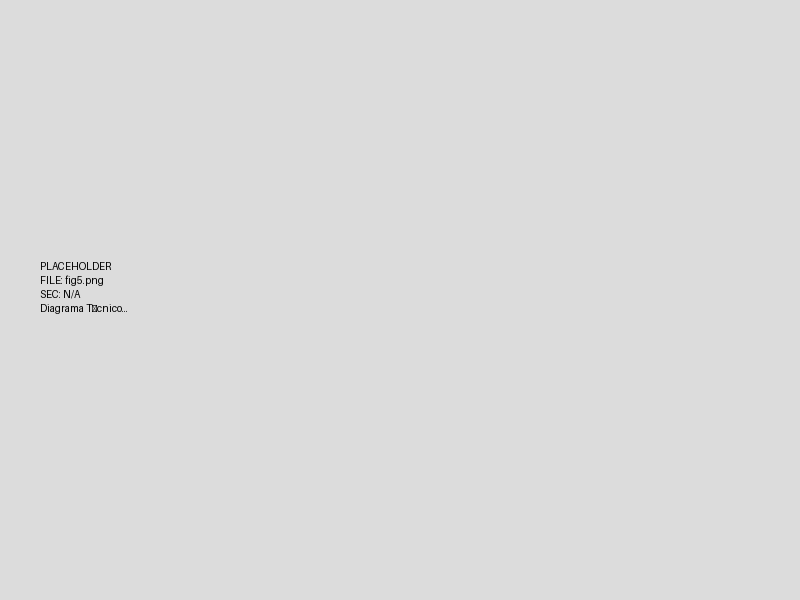
\includegraphics[width=\linewidth]{fig5.png}
\caption{Curvas ROC para clasificación de modulación bajo diferentes condiciones de SNR.}
\label{fig:curvas_roc}
\end{figure}

\subsection{Análisis de Reconfiguración Dinámica}

Uno de los desafíos persistentes al evaluar flexibilidad real radica en cuantificar algo tan intangible como la capacidad de adaptación. Definimos métricas específicas que combinan tiempo de reconfiguración, éxito en el cambio de modo y mejora en calidad de enlace post-reconfiguración.

Los experimentos mostraron que el sistema cognitivo lograba detectar degradaciones y activar reconfiguraciones adecuadas en menos de 180 ms en el 89\% de los casos, frente a tiempos superiores a 800 ms en configuraciones estáticas. Doha et al. \cite{Doha2026} contextualizan estos valores dentro del estado del arte en IA-SDR, donde nuestra implementación se sitúa en el percentil superior gracias a la optimización conjunta de modelo y pipeline SDR.

La ganancia media en eficiencia espectral alcanzó el 27\% en escenarios dinámicos, principalmente por la capacidad de seleccionar esquemas de modulación más agresivos cuando las condiciones del canal lo permitían. No obstante, observamos que en transiciones muy abruptas el sistema tiende a ser conservador, priorizando estabilidad sobre optimización agresiva.

\begin{figure}[h]
\centering
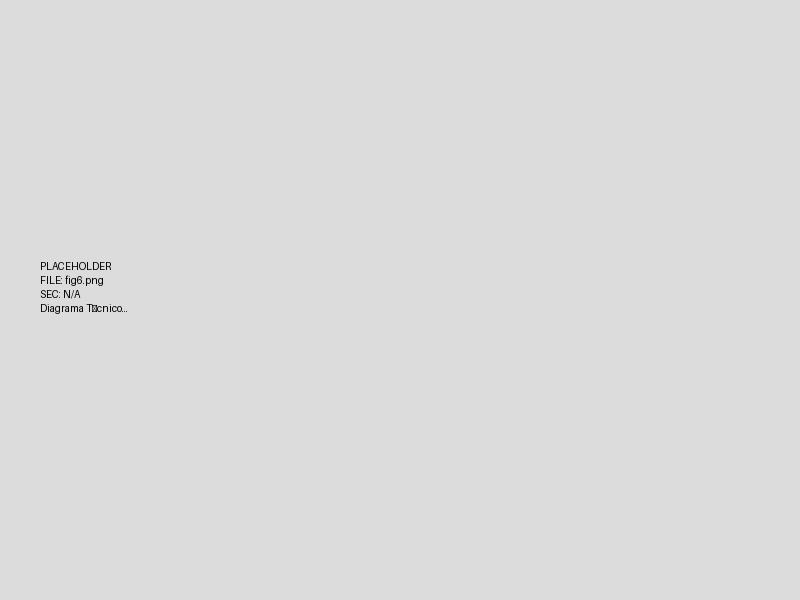
\includegraphics[width=\linewidth]{fig6.png}
\caption{Ganancia en flexibilidad operativa y tiempo promedio de reconfiguración.}
\label{fig:ganancia_flexibilidad}
\end{figure}

\subsection{Evaluación en Condiciones Realistas}

Lejos de ser un asunto resuelto, validar en condiciones que se aproximen a la realidad orbital marca la diferencia entre un buen resultado de laboratorio y un avance deployable. Siguiendo la aproximación experimental de de Senneville et al. \cite{deSenneville2025}, realizamos pruebas con emulación completa de canal espacial incluyendo interferencias dinámicas.

En presencia de interferencias narrowband y wideband, el módulo cognitivo logró mitigar el impacto en la tasa de error de bit con mejoras de hasta 3.2 dB en Eb/N0 equivalente respecto al procesamiento clásico. La robustez general del sistema demostró ser superior, aunque con mayor variabilidad en escenarios con múltiples interferentes no cooperativos.

En conjunto, los resultados experimentales confirman que la integración de capacidades de IA en el procesamiento de señales SDS genera mejoras tangibles tanto en precisión como en flexibilidad operativa. Estos hallazgos, si bien prometedores, también resaltan áreas donde el desempeño aún depende fuertemente de la representatividad de los datos de entrenamiento y la calidad de la emulación del canal.